\documentclass{article}
\usepackage[top=0.2in, bottom=0.1in,left=1.5cm,right=1.5cm]{geometry}
\usepackage{graphicx}
\usepackage{background}

\SetBgScale{1}
\SetBgAngle{0}
\SetBgColor{black}
\SetBgContents{\rule{.5pt}{\paperheight} \rule{.5pt}{\paperheight} 
\qquad \qquad \qquad \qquad \qquad \qquad \qquad \qquad \qquad 
\qquad \qquad \qquad \qquad \qquad \qquad \qquad \qquad \qquad 
\qquad \qquad \qquad \qquad \qquad \qquad \qquad \quad \quad \, \rule{.5pt}{\paperheight} \rule{.5pt}{\paperheight}
}

\begin{document}

\hrule  
\vspace{0.1in}
\includegraphics[width=4cm]{chalk_logo.png}
\huge{ \textbf{CB02 - Switching Power Supply}} 
\vspace{0.05in}
\hrule 
\vspace{0.05in}


\mbox{
\begin{minipage}[t]{0.4\linewidth}
\vspace{0pt}
\large
\textbf{Features and Benefits}
\normalsize
\begin{itemize}
\item Wide input range [5v-18v]
\item High current(1.0A) output
\item Stable 5V output +-2\%
\item Multiple protection schemes
\item Current and Temperature sense via space saving I2C
\item I2C reports current, voltage, power, and temperature
\item Alert pin signals overcurrent condition
\item Soft-startup and current limit
\item Extreme effeciency of up to 95\%
\item Switching frequency of 500kHz lies outside many signal bandwidths
\item Enable provides true enable/disable functionality
\end{itemize}
\end{minipage}

\vrule
\vspace{0.3in}

\begin{minipage}[t]{0.5\linewidth}
\vspace{0pt}
\large{\textbf{Descritpion}} 
\\

\normalsize
CB02 is a 1.0 ampere step down power supply.  It is a fully contained buck regulator with wide input range and is able to maintain an extremely high efficiency over the whole input voltage range [87-95\%]. In addition, the voltage regulation is stable over rated temperature range. \\
CB02 provides a soft-startup of 2.4 m, and a programmable ALERT pin for overcurrent or undervoltage. In addition there is an ENABLE line which allows disconnection of the output from the input. This also turns off the internal regulator. The shutdown current is very small [in the microA range].\\
Switching regulator contains a number of protection features such as thermal shutdown, overvoltage and undervoltage reset and current limit. In addition separate temperature and current sensors are provided on the same I2C bus. The current sensor is intelligent and provides voltage, current and power metrics on supply output. The current sensor is powered from a separate linear regulator. \\
There are also two LEDs providing diagnostic outputs: one for power applied, the other for output voltage available. This allows an easy cursory glance to tell if a power supply is powered and/or enabled and supplying voltage. 

\end{minipage}
} %end mbox
\\
\hspace{0.3in}
\hrule
\hspace{0.3in}
\begin{center} 
\large{\textbf{Typical Application}}
\end{center}
\begin{center}
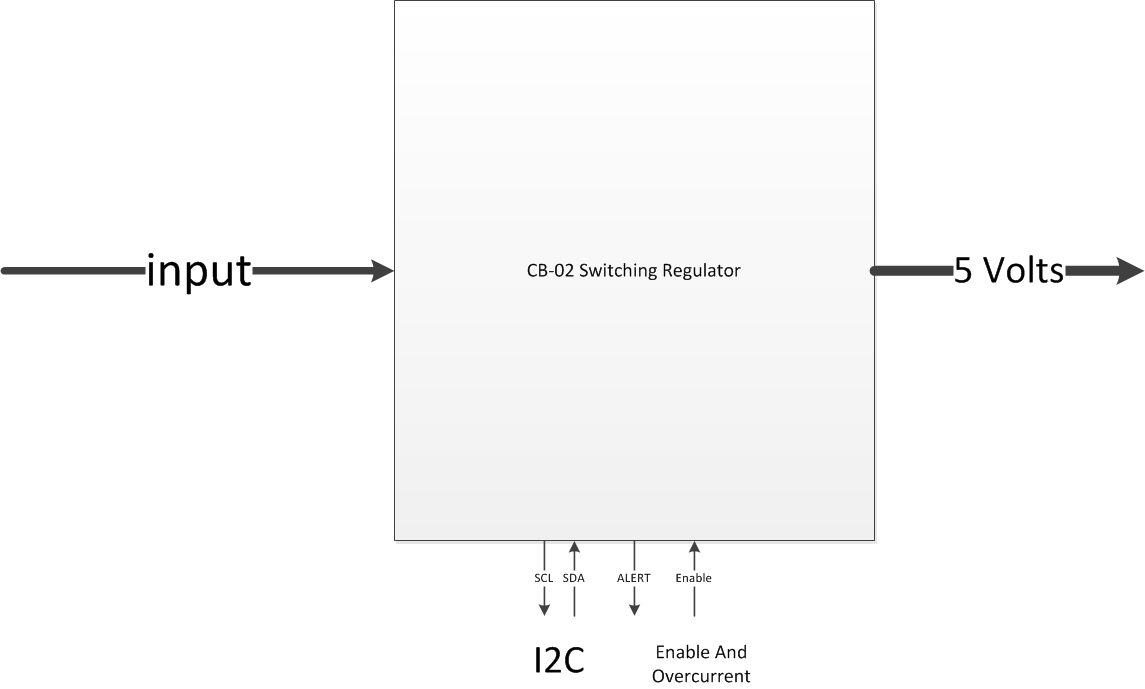
\includegraphics[width=6in]{CB02_block.png}
\end{center}
\hrule
\newpage
\large{\textbf{Power \& Thermal Characteristics}} \\
%page 2!
\begin{center}
\begin{tabular}{|l | l |c| c|c|c|c|}
\hline
Characteristics & Symbol &Test Conditions & Min & Typ & Max & Units \\ \hline
Functional Input Voltage& $V_{in}$& & 5.4&12&18&V \\ \hline 
Output Voltage & $V_{out}$ & Over input voltage& 4.85 & 4.95 & 5.0 & V \\ \hline
Output Current & $I_{max}$ &Output current& 0 & 1.0& 1.2 &A \\ \hline
Switching Frequency& $F_{sw}$ &480 & &500&520& kHz \\ \hline
Output Voltage Ripple &$V_{ripple}$& Full load & 0& 20&75&mV \\ \hline
Output Inductor Current Ripple &$I_{ripple}$& Full load  PtP& &265&& mA \\\hline
Output current Slew Rate&$I_{slew}$& Full load&&318&& A/ms \\ \hline
Heating &$T_{heat}$ & Full load & 6&10&12& K \\ \hline
Efficiency & Eff &Vin=12V, Iout=1.0A& & 95 &  & \% \\\hline
Total Idle Consumption  & $I_{idle}$ & $I_{out}=0$, over full $V_{in}$ range & 10 & 16 & 25& mA \\ \hline 
\hline
\end{tabular}
\end{center}
\large{\textbf{Electrical \& Logical Characteristics}} \\
\begin{center}
\begin{tabular}{|l | l |c| c|c|c|c|}
\hline
Characteristics & Symbol &Test Conditions & Min & Typ & Max & Units \\ \hline
Functional Input Voltage& $V_{in}$& & 3.5&12&18&V \\ \hline 
Bus Voltage Accuracy& $Acc_{bvol}$& Over full $V_{in}$ range&  -1&0.5&1&\% \\ \hline
Shunt Voltage Accuracy&$Acc_{svol}$& Over full $I_{load}$ range&-1.25&0.6&1.25&\% \\ \hline
Output Current Accuracy&$Acc_{iout}$&Over full range& -2&0.5&2&\% \\ \hline
Temperature Accuracy &$Acc_{T}$&Over full range& -2 &0&2& K\\ \hline
Enable Line Consumption &$I_{enable}$& Enable = HIGH, steady-state & 1 & 1.1 &1.2& mA\\ \hline
\hline
\end{tabular}
\end{center}
\large{\textbf{General Usage}} \\
CB02 is a fully enclosed switching power supply module. To enable operation you need to connect power to either the high side terminals or the Vin pin/GND, and push ENABLE high. The ENABLE pin controls two things: the input power switch and the LDO regulator for circuitry. The regulator starts first and it powers both the temperature sensor and the outpure current sensor. It is recomended that you program the output current sensors at this point to report overcurrent conditions.  A couple ms later the input power switch turns on and the switching controller initializes[2.4ms]. At this point the part will be fully-on and stabilizing voltage.

Temperature and current data is available via either standard or high speed I2C. Addresses are summarized in the table that follows. To enable high speed please read the datasheets of the sensors; by default only the standard I2C speeds are aviable [100-400 kHz].

It is highly recomend that you re-program the current sensor as part of your boot-up routine. The overcurrent registers are volatile and will reset every time the enable pin is pulled low. As such it is recomended that you reprogram the overcurret at 1.4A, and monitor the ALERT pin in an ISR. Then in the ISR read the value of the overcurrent and immidiately disable the part by pulling ENABLE low. Diagnose and repair the overcurrent condition, after which you can re-enable the part.

\begin{tabular}{|l|c|c|}
%\caption{Adress alocation based on CB02 number}
\hline
Sensor Type &CB02-01 &CH02-02\\ \hline
Temperature Sensor Address & 68 &73\\ \hline
Current Sensor Address&   69&  79 \\ \hline
\hline
\end{tabular}


\end{document}


